% ===================================================================
%  Health Data in South Korea - an introduction
%  Siho Park, KDI School of Public Policy and Management
%  Compile with XeLaTeX (Korean terms require kotex)
% ===================================================================

\documentclass[aspectratio=169,11pt]{beamer}

\usepackage{kotex}          % Korean terms
\usepackage{booktabs}
\usepackage{tabularx}
\usepackage{array}
\usepackage{tikz}
\usetikzlibrary{positioning}

\usepackage{hyperref}
\hypersetup{colorlinks=true, linkcolor=., urlcolor=kdgreenmid, citecolor=kdgreenmid}

% ------------------------------------------------------------------
%  Colors
% ------------------------------------------------------------------
\definecolor{kdgreen}{HTML}{0E4430}     % primary, dark green
\definecolor{kdgreenmid}{HTML}{1B7A57}  % secondary, for bullets and links
\definecolor{kdaccent}{HTML}{C2601C}    % accent, burnt orange
\definecolor{kdgray}{HTML}{55605A}
\definecolor{kdlight}{HTML}{EDF3EF}
\definecolor{kdrule}{HTML}{C7D7CD}

% ------------------------------------------------------------------
%  Theme
% ------------------------------------------------------------------
\usetheme{default}
\usefonttheme{professionalfonts}
\setbeamertemplate{navigation symbols}{}

\setbeamercolor{structure}{fg=kdgreen}
\setbeamercolor{frametitle}{fg=kdgreen, bg=white}
\setbeamercolor{framesubtitle}{fg=kdgray}
\setbeamercolor{title}{fg=white}
\setbeamercolor{normal text}{fg=black!88}
\setbeamercolor{itemize item}{fg=kdgreenmid}
\setbeamercolor{itemize subitem}{fg=kdgray}
\setbeamercolor{block title}{fg=white, bg=kdgreen}
\setbeamercolor{block body}{fg=black!88, bg=kdlight}
\setbeamercolor{alerted text}{fg=kdaccent}

\setbeamerfont{frametitle}{size=\large, series=\bfseries}
\setbeamerfont{framesubtitle}{size=\small, series=\mdseries}
\setbeamerfont{title}{size=\LARGE, series=\bfseries}
\setbeamerfont{block title}{size=\small, series=\bfseries}
\setbeamerfont{block body}{size=\small}
\setbeamerfont{itemize/enumerate subbody}{size=\small}
\setbeamerfont{itemize/enumerate subsubbody}{size=\footnotesize}
\setbeamerfont{footline}{size=\tiny}

\setbeamertemplate{itemize item}{\raisebox{0.12ex}{\scriptsize$\blacktriangleright$}}
\setbeamertemplate{itemize subitem}{\raisebox{0.15ex}{\tiny$-$}}
\setbeamertemplate{section in toc}{%
  \leavevmode\color{kdgreen}\textbf{\inserttocsectionnumber.}~\inserttocsection\par}

\makeatletter
\setbeamertemplate{frametitle}{%
  \vspace*{0.45em}%
  \begin{beamercolorbox}[wd=\paperwidth, leftskip=0.9cm, rightskip=0.9cm]{frametitle}%
    \usebeamerfont{frametitle}\insertframetitle\par
    \ifx\insertframesubtitle\@empty\else
      \vspace{1pt}{\usebeamerfont{framesubtitle}\usebeamercolor[fg]{framesubtitle}\insertframesubtitle\par}%
    \fi
    \vspace{2pt}{\color{kdaccent}\rule{2.1cm}{1.4pt}}
  \end{beamercolorbox}%
}
\makeatother

\setbeamertemplate{footline}{%
  \hbox{%
  \begin{beamercolorbox}[wd=\paperwidth, ht=2.6ex, dp=1.4ex, leftskip=0.9cm, rightskip=0.9cm]{}%
    \usebeamerfont{footline}\color{kdgray}%
    \insertshorttitle\hfill\insertframenumber\,/\,\inserttotalframenumber
  \end{beamercolorbox}}%
}

% Section divider
\AtBeginSection[]{%
\begin{frame}[plain, noframenumbering]
  \begin{tikzpicture}[remember picture, overlay]
    \fill[kdgreen] (current page.north west) rectangle (current page.south east);
    \node[anchor=south west, text width=0.72\paperwidth, align=left]
      at ([xshift=2.2cm, yshift=0.45cm]current page.west)
      {\color{kdaccent}\large\bfseries SECTION \insertsectionnumber};
    \node[anchor=north west, text width=0.72\paperwidth, align=left]
      at ([xshift=2.2cm, yshift=0.25cm]current page.west)
      {\color{white}\Huge\bfseries\insertsection};
    \draw[kdaccent, line width=2pt]
      ([xshift=1.5cm, yshift=1.5cm]current page.west) --
      ([xshift=1.5cm, yshift=-1.2cm]current page.west);
  \end{tikzpicture}
\end{frame}}

% Helper: compact table rows
\newcommand{\hl}[1]{\textbf{\color{kdgreen}#1}}
\newcommand{\han}[1]{{\footnotesize\color{kdgray}(#1)}}

% ------------------------------------------------------------------
\title{Health Data in South Korea}
\subtitle{A practical introduction to survey, claims, and registry data}
\author{Siho Park}
\institute{KDI School of Public Policy and Management}
\date{\today}
\titlegraphic{}

\begin{document}

% ---------------------------------------------------- Title page
\begin{frame}[plain, noframenumbering]
  
\begin{tikzpicture}[remember picture, overlay]
    \fill[kdgreen] (current page.north west) rectangle (current page.south east);
    \fill[kdaccent] ([yshift=-3.05cm]current page.north west)
      rectangle ([yshift=-3.12cm]current page.north east);
    \node[anchor=north west, text width=0.86\paperwidth, align=left]
      at ([xshift=1.4cm, yshift=-1.5cm]current page.north west)
      {\color{white}\Huge\bfseries Health Data in South Korea};
    \node[anchor=north west, text width=0.80\paperwidth, align=left]
      at ([xshift=1.4cm, yshift=-3.6cm]current page.north west)
      {\color{white!80}\large A practical introduction to survey, claims, and registry data};
    \node[anchor=south west, text width=0.80\paperwidth, align=left]
      at ([xshift=1.4cm, yshift=1.1cm]current page.south west)
      {\color{white}\large\bfseries Siho Park\\[0.3em]
       \color{white!75}\normalsize\mdseries KDI School of Public Policy and Management\\[0.15em]
       \color{white!65}\footnotesize\mdseries \today};
  \end{tikzpicture}
\end{frame}

% ---------------------------------------------------- Motivation
\begin{frame}{Why Korean health data?}
  \begin{itemize}
    \setlength{\itemsep}{8pt}
    \item \hl{One insurer for the whole country.} National Health Insurance has covered
          essentially everyone since 1989, and the separate insurance societies were
          merged into a single insurer in 2000.
    \item \hl{People do not disappear.} Records follow the same person across jobs,
          regions, and providers, without the gaps that arise when people switch insurers.
    \item \hl{Screening is national and routine.} Most adults are invited to a free or
          nearly free health check every two years, which produces biomarkers for
          millions of people, not just for patients.
  \end{itemize}
  \vspace{1pt}
  \begin{block}{}
    A rare combination: administrative data at population scale, alongside
    national surveys with the detail that administrative data lack.
  \end{block}
  \vspace{-4pt}
\end{frame}

% ---------------------------------------------------- Roadmap
\begin{frame}{Four datasets in this talk}
  \vspace{2pt}
  \renewcommand{\arraystretch}{1.5}
  \begin{tabularx}{\textwidth}{@{}l>{\raggedright\arraybackslash}X@{}}
    \toprule
    \hl{NHIS claims} & National health insurance claims data \\
    \hl{K-CURE} & Cancer registry data linked to claims, screening,
      and death \\
    \hl{KNHANES} & National survey with a physical examination and a
      nutrition interview \\
    \hl{KHPS} & Household panel survey with
      visit-level health care use and costs \\
    \bottomrule
  \end{tabularx}
  \vspace{8pt}

\end{frame}

% ---------------------------------------------------- The trade-off
\begin{frame}{The trade-off that organizes everything}
  \framesubtitle{Scale buys rare outcomes; surveys buy context}
  \vspace{-6pt}
  \begin{center}
  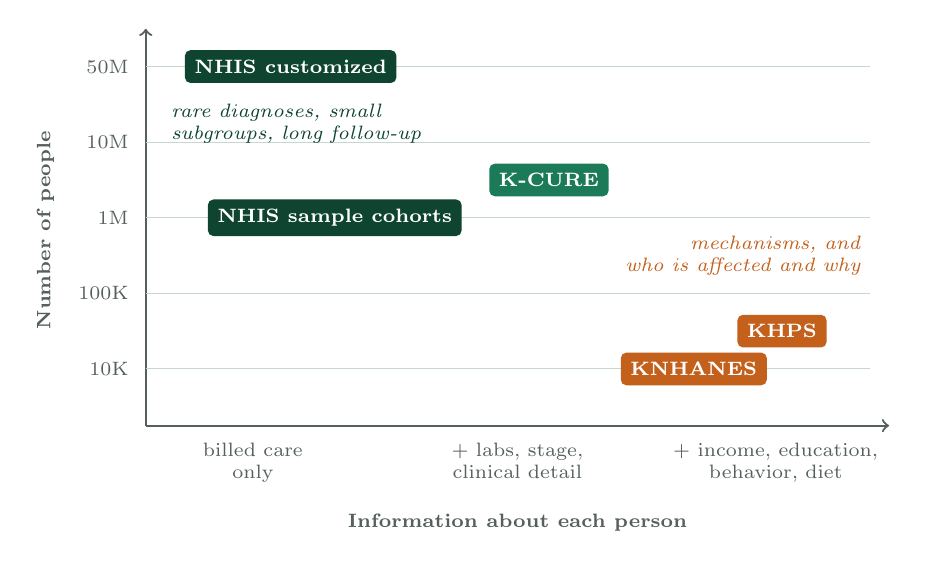
\begin{tikzpicture}[scale=0.80, every node/.style={font=\footnotesize}]
    % axes
    \draw[->, thick, kdgray] (0,0) -- (11.8,0);
    \draw[->, thick, kdgray] (0,0) -- (0,6.3);
    \node[rotate=90, anchor=south, font=\scriptsize\bfseries, kdgray] at (-1.3,3.1) {Number of people};
    \node[anchor=north, font=\scriptsize\bfseries, kdgray] at (5.9,-1.25) {Information about each person};

    % y ticks
    \foreach \y/\lab in {0.9/10K, 2.1/100K, 3.3/1M, 4.5/10M, 5.7/50M}{
      \draw[kdrule] (0,\y) -- (11.5,\y);
      \node[anchor=east, font=\scriptsize, kdgray] at (-0.12,\y) {\lab};}

    % x annotations
    \node[anchor=north, font=\scriptsize, kdgray, text width=2.6cm, align=center] at (1.7,-0.12) {billed care\\only};
    \node[anchor=north, font=\scriptsize, kdgray, text width=2.6cm, align=center] at (5.9,-0.12) {+ labs, stage,\\clinical detail};
    \node[anchor=north, font=\scriptsize, kdgray, text width=3.4cm, align=center] at (10.0,-0.12) {+ income, education,\\behavior, diet};

    % points
    \node[fill=kdgreen, text=white, rounded corners=2pt, inner sep=3.5pt, font=\scriptsize\bfseries]
      at (2.3,5.7) {NHIS customized};
    \node[fill=kdgreen, text=white, rounded corners=2pt, inner sep=3.5pt, font=\scriptsize\bfseries]
      at (3.0,3.3) {NHIS sample cohorts};
    \node[fill=kdgreenmid, text=white, rounded corners=2pt, inner sep=3.5pt, font=\scriptsize\bfseries]
      at (6.4,3.9) {K-CURE};
    \node[fill=kdaccent, text=white, rounded corners=2pt, inner sep=3.5pt, font=\scriptsize\bfseries]
      at (10.1,1.5) {KHPS};
    \node[fill=kdaccent, text=white, rounded corners=2pt, inner sep=3.5pt, font=\scriptsize\bfseries]
      at (8.7,0.9) {KNHANES};

    % annotations
    \node[anchor=west, font=\scriptsize\itshape, kdgreen, text width=3.4cm]
      at (0.25,4.8) {rare diagnoses, small\\subgroups, long follow-up};
    \node[anchor=east, font=\scriptsize\itshape, kdaccent, text width=3.2cm, align=right]
      at (11.5,2.7) {mechanisms, and\\who is affected and why};
  \end{tikzpicture}
  \end{center}
\end{frame}

% ---------------------------------------------------- Agenda
\begin{frame}{Outline}
  \vspace{14pt}
  \begin{columns}[T]
    \begin{column}{0.50\textwidth}
      \large
      \tableofcontents
    \end{column}
    \begin{column}{0.46\textwidth}
      \begin{block}{Two documentation sites}
        I maintain English documentation for the two administrative sources,
        and this talk draws on it.
        \vspace{4pt}
        \begin{itemize}\small
          \item \href{https://siho-park.github.io/nhis-documentation/}{NHIS Data Documentation}
          \item \href{https://siho-park.github.io/kcure-documentation/}{K-CURE Data Documentation}
        \end{itemize}
      \end{block}
    \end{column}
  \end{columns}
\end{frame}

% ===================================================================
\section{NHIS claims data}
% ===================================================================

\begin{frame}{Where the data come from}
  \framesubtitle{Every record is a by-product of running the insurance program}
  \begin{itemize}
    \setlength{\itemsep}{8pt}
    \item \hl{Enrolling people} $\rightarrow$ eligibility records: insurance type, premium,
          disability, district of residence.
    \item \hl{Paying claims} $\rightarrow$ claims records: diagnoses, procedures, drugs, and
          what the insurer and the patient each paid.
    \item \hl{Running the screening program} $\rightarrow$ examination results: blood pressure,
          cholesterol, glucose, body measurements, and a lifestyle questionnaire.
    \item \hl{Linking the death register} $\rightarrow$ date and cause of death from the
          national statistics agency.
  \end{itemize}
  \vspace{4pt}
  \begin{block}{Why this framing matters}
    The data measure what the program needed to record. Care that generates no
    claim, and income that sets no premium, simply are not there.
  \end{block}
\end{frame}

\begin{frame}{What is inside}
  \vspace{2pt}
  \renewcommand{\arraystretch}{1.35}
  {\small
  \begin{tabularx}{\textwidth}{@{}l l >{\raggedright\arraybackslash}X@{}}
    \toprule
    \textbf{Records} & \textbf{Unit} & \textbf{Main content} \\
    \midrule
    Eligibility \han{자격} & person-year & Insurance type, premium decile, disability, residence \\
    Claims \han{진료} & claim and line & Diagnoses, procedures, drugs, spending, length of stay \\
    Screening \han{건강검진} & examination & Blood pressure, lipids, glucose, BMI, smoking, drinking \\
    Death \han{사망} & person & Date and cause of death \\
    Long-term care \han{장기요양} & application, claim & Care grade assessment and use, from 2008 \\
    Providers \han{요양기관} & provider-year & Type, size, and location of the facility \\
    \bottomrule
  \end{tabularx}}
  \vspace{7pt}

  {\small Claims split into four linked tables: the claim itself, the service
  lines on it, the diagnoses on it, and outpatient prescriptions.}
\end{frame}

\begin{frame}{The screening data are the underrated part}
  \begin{columns}[T]
    \begin{column}{0.56\textwidth}
      \begin{itemize}
        \setlength{\itemsep}{7pt}
        \item Most adults are invited every two years; non-office workers every year.
        \item Gives \hl{objective health measures for people who are not sick} ---
              the counterfactual that claims data cannot provide.
        \item Includes a self-reported questionnaire on smoking, drinking,
              and exercise, so behavior and biomarkers sit on the same record.
        \item Repeated over two decades for the same people.
      \end{itemize}
    \end{column}
    \begin{column}{0.42\textwidth}
      \begin{block}{Useful to know}
        \begin{itemize}\small
          \item Screening content changed in 2009 and 2018; the questionnaire items
                are not comparable across all years.
          \item Cancer screening is a separate program and is \emph{not} in the
                standard claims or screening tables.
        \end{itemize}
      \end{block}
    \end{column}
  \end{columns}
\end{frame}

\begin{frame}{Who is inside: the ready-made samples}
  \vspace{-2pt}
  \renewcommand{\arraystretch}{1.3}
  {\footnotesize
  \begin{tabularx}{\textwidth}{@{}l >{\raggedright\arraybackslash}X r l@{}}
    \toprule
    \textbf{Database} & \textbf{Population} & \textbf{Size} & \textbf{Years} \\
    \midrule
    National Sample Cohort \han{표본코호트} & Enrolled throughout 2006, all ages & 1,000,000 & 2002--2023 \\
    Health Screening Cohort \han{건강검진코호트} & Aged 40--79 and screened in 2002 or 2003 & 514,866 & 2002--2023 \\
    Senior Cohort \han{노인코호트} & Aged 60--80 and enrolled in 2008 & 511,953 & 2002--2023 \\
    Low-Risk Sample \han{저위험 표본} & Used medical care in 2014--2023 & 1,000,000 & 2014--2023 \\
    \bottomrule
  \end{tabularx}}
  \vspace{7pt}

  \begin{itemize}\small
    \setlength{\itemsep}{4pt}
    \item The National Sample Cohort is the usual default: all ages, refreshed with
          newborns, and including Medical Aid beneficiaries.
    \item The Screening Cohort is richer on screening, but is a closed, aging cohort
          of people already screened --- not the general population.
    \item \hl{No household or family links} in any of them.
  \end{itemize}
\end{frame}

\begin{frame}{Who is inside: the customized extract}
  \begin{itemize}
    \setlength{\itemsep}{9pt}
    \item A \hl{customized research DB} \han{맞춤형연구DB} is built from the full national
          database to match an approved protocol.
    \item It can cover \hl{everyone who meets the study criteria}, not a sample ---
          tens of millions of people.
    \item This is what makes rare outcomes feasible: a condition affecting one in
          ten thousand gives a handful of cases in a one-million sample and
          thousands in the full population.
    \item It is also the only route to diagnoses that are \hl{masked in the sample
          databases}, including all mental and behavioral disorders, pregnancy and
          childbirth, and breast and genital cancers.
    \item The cost is a longer review, a higher fee, and analysis only at an
          NHIS analysis center.
  \end{itemize}
\end{frame}

\begin{frame}{What you can study}
  \begin{columns}[T]
    \begin{column}{0.48\textwidth}
      \textbf{\color{kdgreen}Natural fits}
      \begin{itemize}\small
        \setlength{\itemsep}{6pt}
        \item Health care utilization and spending, at the visit, episode, or
              annual level
        \item Policy evaluation using age, date, or eligibility cutoffs built
              into the program
        \item Disease incidence, progression, and mortality over long horizons
        \item Provider behavior and regional variation in treatment
        \item Drug utilization and safety
      \end{itemize}
    \end{column}
    \begin{column}{0.48\textwidth}
      \textbf{\color{kdaccent}What the scale buys}
      \begin{itemize}\small
        \setlength{\itemsep}{6pt}
        \item Rare diagnoses and rare adverse events
        \item Narrow subgroups: one age, one region, one occupation
        \item Precisely estimated effects at discontinuities, where only
              observations near the cutoff count
        \item Mortality as an outcome, which needs many person-years
      \end{itemize}
    \end{column}
  \end{columns}
\end{frame}

\begin{frame}{What it cannot tell you}
  \begin{itemize}
    \setlength{\itemsep}{7pt}
    \item \hl{No income and no education.} The premium decile stands in for income,
          but premiums come from wages for employees and from income and property
          for the self-employed, so the same decile means different things across groups.
    \item \hl{Non-covered services are invisible} \han{비급여}. Services patients pay for
          entirely out of pocket are never billed to the insurer, so any measure of
          total spending is incomplete, and incomplete by different amounts across
          conditions and years.
    \item \hl{A diagnosis code is a billing code.} It records what justified a claim,
          not a confirmed diagnosis.
    \item \hl{No families and no households}, in the sample databases.
    \item \hl{Identifiers do not travel.} Each release has its own pseudonymized ID,
          so people cannot be followed across databases or linked to outside data.
  \end{itemize}
\end{frame}

\begin{frame}{Getting access}
  \begin{columns}[T]
    \begin{column}{0.49\textwidth}
      \textbf{\color{kdgreen}The process}
      \begin{itemize}\small
        \setlength{\itemsep}{5pt}
        \item Apply at \href{https://nhiss.nhis.or.kr}{nhiss.nhis.or.kr}
        \item IRB approval and protocol, \hl{in Korean}
        \item Research summary read by a committee, \hl{in Korean}
        \item Principal investigator must be a Korean national living in Korea
        \item Fee follows the period requested, not the days used; reduced 80\% for
              a thesis, 50\% for academic research
      \end{itemize}
    \end{column}
    \begin{column}{0.49\textwidth}
      \textbf{\color{kdaccent}Working with it}
      \begin{itemize}\small
        \setlength{\itemsep}{5pt}
        \item You never receive the data; analysis runs on NHIS servers
        \item Sample databases: remote connection from your own computer
        \item Customized DB: in person at an analysis center
        \item \hl{Both work only while you are physically in Korea}
        \item Results leave only after an export review
      \end{itemize}
    \end{column}
  \end{columns}
  \vspace{4pt}
  \begin{block}{For researchers based abroad}
    Everything up to the analysis can be done online. The analysis itself needs a
    visit, so set the period of use around the trip.
  \end{block}
\end{frame}

% ===================================================================
\section{K-CURE cancer data}
% ===================================================================

\begin{frame}{What K-CURE is}
  \framesubtitle{The national cancer registry, linked to everything else}
  \begin{itemize}
    \setlength{\itemsep}{8pt}
    \item A data portal run by the Ministry of Health and Welfare that releases the
          \hl{Korea Central Cancer Registry} \han{중앙암등록본부} joined to administrative records.
    \item The registry says \hl{who was diagnosed, with which cancer, when, and at
          what stage}. The linked files say what care came before and after.
    \item The main product, the \hl{Cancer Public Library} \han{암 공공 라이브러리},
          covers about 2.26 million registered cancer patients.
  \end{itemize}
  \vspace{4pt}
  \begin{block}{Why not just use claims?}
    In claims data a cancer is a billing code, with no stage, no histology, and an
    uncertain date. A registry record is a reported cancer with a diagnosis date
    and a stage --- which is exactly what survival and early-detection research needs.
  \end{block}
\end{frame}

\begin{frame}{What is inside}
  \vspace{2pt}
  \renewcommand{\arraystretch}{1.35}
  {\small
  \begin{tabularx}{\textwidth}{@{}l >{\raggedright\arraybackslash}X@{}}
    \toprule
    \textbf{Group} & \textbf{Content} \\
    \midrule
    Registry \han{RGST} & One row per registered cancer: site, histology, diagnosis date,
      SEER summary stage. Two cancers means two rows. \\
    Death & Date and cause of death \\
    Eligibility & Insurance type and premium, one row per person-year \\
    Claims & Claim, service line, diagnosis, and outpatient prescription \\
    Health checkup & Examination results and the lifestyle questionnaire \\
    Cancer screening & Stomach, breast, colorectal, cervical, and liver, separately \\
    COVID-19 & Confirmed cases and vaccinations \\
    \bottomrule
  \end{tabularx}}
  \vspace{6pt}

  {\small All tables join on one person identifier. Cancer screening results are
  here, where they are \emph{not} in the standard NHIS sample databases.}
\end{frame}

\begin{frame}{Three ways to get it}
  \vspace{-2pt}
  \renewcommand{\arraystretch}{1.25}
  {\footnotesize
  \begin{tabularx}{\textwidth}{@{}l >{\raggedright\arraybackslash}X >{\raggedright\arraybackslash}X >{\raggedright\arraybackslash}X@{}}
    \toprule
    & \textbf{Customized} \han{맞춤형} & \textbf{Site sample} \han{표본} & \textbf{Staging sample} \\
    \midrule
    Who & Every registered cancer, 2012--2022 & About 20\% of one cancer site & About 10\% of one site \\
    Sites & All & Stomach, breast, colorectal, liver, lung, pancreas & Stomach, breast, colorectal, liver, lung \\
    Stage & Summary stage & Summary stage & Tumor size, nodes, metastasis, grade, TNM \\
    Variables & What you request & Fixed shorter list & Fixed list \\
    Analyzed & At a safe-use center, in person & Remote virtual desktop & Remote virtual desktop \\
    Wait & $\sim$3 months & $\sim$1 month & $\sim$1 month \\
    \bottomrule
  \end{tabularx}}
  \vspace{6pt}

  {\small A study of thyroid, cervical, or hematologic cancer, or of several sites
  together, needs the customized extract.}
\end{frame}

\begin{frame}{What you can study}
  \begin{columns}[T]
    \begin{column}{0.48\textwidth}
      \textbf{\color{kdgreen}Questions it answers well}
      \begin{itemize}\small
        \setlength{\itemsep}{6pt}
        \item Survival by stage, site, and year of diagnosis
        \item Whether screening shifts cancers toward earlier stages
        \item Treatment patterns and how they vary across providers and regions
        \item The cost of cancer care, and who bears it
        \item Socioeconomic and regional disparities in stage at diagnosis
      \end{itemize}
    \end{column}
    \begin{column}{0.48\textwidth}
      \textbf{\color{kdaccent}Limits to plan around}
      \begin{itemize}\small
        \setlength{\itemsep}{6pt}
        \item Cancer patients only --- there is no healthy comparison group
        \item Starts in 2012
        \item You cannot link further person-level data yourself; a linkage has to be
              built into the project from the start
        \item Some items, such as single-year age, are released only with a
              justification
      \end{itemize}
    \end{column}
  \end{columns}
  \vspace{5pt}
  {\small Access conditions resemble the NHIS: Korean principal investigator,
  IRB approval, analysis in a controlled environment, and export review.}
\end{frame}

% ===================================================================
\section{KNHANES}
% ===================================================================

\begin{frame}{Korea National Health and Nutrition Examination Survey}
  \framesubtitle{국민건강영양조사 --- run by the Korea Disease Control and Prevention Agency}
  \begin{itemize}
    \setlength{\itemsep}{8pt}
    \item A nationally representative survey, running annually, of roughly
          \hl{10,000 people a year} across all ages.
    \item Three components collected for the same person:
      \begin{itemize}
        \item \hl{Health interview}: conditions, health care use, education, occupation, household
        \item \hl{Health examination}: blood pressure, height and weight, blood and urine
              tests, and depending on the year, vision, hearing, lung function, and bone density
        \item \hl{Nutrition survey}: a 24-hour dietary recall and food frequency, done at home
      \end{itemize}
    \item \hl{Cross-sectional}: a fresh sample each year, not a panel.
  \end{itemize}
  \vspace{4pt}
  \begin{block}{The distinctive feature}
    Measured values, not reported ones. You can see who has high blood pressure
    \emph{and does not know it} --- something no claims database can show.
  \end{block}
\end{frame}

\begin{frame}{What you can study, and what you cannot}
  \begin{columns}[T]
    \begin{column}{0.48\textwidth}
      \textbf{\color{kdgreen}Strengths}
      \begin{itemize}\small
        \setlength{\itemsep}{6pt}
        \item National prevalence and long-run trends in obesity, diabetes,
              hypertension, smoking
        \item Diet and nutrition as an exposure, in detail available nowhere else
        \item Undiagnosed and untreated disease
        \item Socioeconomic gradients, since income and education are measured directly
        \item \hl{Free and immediate}: download the microdata from the website
      \end{itemize}
    \end{column}
    \begin{column}{0.48\textwidth}
      \textbf{\color{kdaccent}Limits}
      \begin{itemize}\small
        \setlength{\itemsep}{6pt}
        \item Too small for rare conditions or narrow subgroups
        \item No panel: you cannot follow a person over time
        \item No claims, so health care use is self-reported and coarse
        \item Survey weights and the clustered design must be used correctly
        \item Questionnaire items change across waves; pooling years takes care
      \end{itemize}
    \end{column}
  \end{columns}
  \vspace{6pt}
  {\small Often the fastest way to establish a descriptive fact that motivates a
  project, before committing to an administrative data application.}
\end{frame}

% ===================================================================
\section{Korea Health Panel Study}
% ===================================================================

\begin{frame}{Korea Health Panel Study}
  \framesubtitle{한국의료패널 --- a household panel on health care use and spending}
  \begin{itemize}
    \setlength{\itemsep}{8pt}
    \item Follows about \hl{7,000 households and 21,000 individuals} over time,
          interviewing the same families repeatedly.
    \item \hl{Sampled at the household level}, so spouses, parents, and children can be
          identified and studied together.
    \item Records health care use at the \hl{visit level} --- outpatient, inpatient, and
          emergency --- with what each visit cost the household.
    \item Collects what administrative data lack: individual and household income,
          educational attainment, private insurance, health behaviors, and
          unmet need.
    \item Note that the panel was redesigned, so the earlier and later waves are
          separate panels rather than one continuous series.
  \end{itemize}
\end{frame}

\begin{frame}{What you can study, and what you cannot}
  \begin{columns}[T]
    \begin{column}{0.48\textwidth}
      \textbf{\color{kdgreen}Strengths}
      \begin{itemize}\small
        \setlength{\itemsep}{6pt}
        \item \hl{Out-of-pocket spending including non-covered care} --- the gap in
              the claims data
        \item Catastrophic health expenditure and financial burden
        \item Unmet medical need, and why people forgo care
        \item Within-family spillovers and household health decisions
        \item Income and health over time, with the same people observed repeatedly
        \item Easy access: sign a consent form and the files are sent to you
      \end{itemize}
    \end{column}
    \begin{column}{0.48\textwidth}
      \textbf{\color{kdaccent}Limits}
      \begin{itemize}\small
        \setlength{\itemsep}{6pt}
        \item Self-reported throughout, including diagnoses and spending
        \item Too small for rare outcomes, and births and deaths are few
        \item Health behaviors recorded in categories rather than continuous amounts
        \item Attrition, as in any long panel
      \end{itemize}
    \end{column}
  \end{columns}
\end{frame}

% ===================================================================
\section{Choosing among them}
% ===================================================================

\begin{frame}{Side by side}
  \vspace{-2pt}
  \renewcommand{\arraystretch}{1.22}
  {\scriptsize
  \begin{tabularx}{\textwidth}{@{}l >{\raggedright\arraybackslash}X >{\raggedright\arraybackslash}X >{\raggedright\arraybackslash}X >{\raggedright\arraybackslash}X@{}}
    \toprule
    & \textbf{NHIS claims} & \textbf{K-CURE} & \textbf{KNHANES} & \textbf{KHPS} \\
    \midrule
    Type & Administrative & Registry + administrative & Survey + exam & Survey panel \\
    People & 1M sample, or the full population & 2.3M cancer patients & $\sim$10,000 per year & $\sim$21,000 \\
    Structure & Long panel, 2002--2023 & Panel, 2012--2022 & Repeated cross-sections & Household panel \\
    Income & Premium decile only & Premium decile only & Measured & Measured \\
    Education & No & No & Yes & Yes \\
    Biomarkers & Screening results & Checkup results & Full examination & No \\
    Diagnoses & Billing codes & Registry, with stage & Self-reported + measured & Self-reported \\
    Spending & Covered care only & Covered care only & No & Including out-of-pocket \\
    Families & No & No & Household roster & Yes, by design \\
    Rare outcomes & Yes & Yes, for cancer & No & No \\
    Access effort & High & High & \hl{Very low} & Low \\
    \bottomrule
  \end{tabularx}}
\end{frame}

\begin{frame}{Which data for which question}
  \vspace{2pt}
  \renewcommand{\arraystretch}{1.45}
  \begin{tabularx}{\textwidth}{@{}>{\raggedright\arraybackslash}X l@{}}
    \toprule
    \textbf{If your question is about\ldots} & \textbf{Start with} \\
    \midrule
    A rare disease, a rare adverse event, or mortality & NHIS customized \\
    A policy with an age or eligibility cutoff & NHIS sample cohort \\
    Cancer survival, stage, or early detection & K-CURE \\
    Prevalence, trends, or undiagnosed disease & KNHANES \\
    Diet, nutrition, or measured risk factors & KNHANES \\
    Out-of-pocket burden or unmet need & KHPS \\
    Families, spouses, or household decisions & KHPS \\
    Long-term care in old age & NHIS sample cohort \\
    \bottomrule
  \end{tabularx}
\end{frame}

\begin{frame}{Practical advice}
  \begin{itemize}
    \setlength{\itemsep}{8pt}
    \item \hl{Use the surveys to design the administrative study.} Establish the
          descriptive fact in KNHANES or KHPS, where data arrive in a day, before
          spending months on an NHIS application.
    \item \hl{Check your case counts before you apply.} A rare condition in a
          one-million sample may not support the analysis you are proposing.
    \item \hl{Write the application and the IRB protocol together}, in Korean. They
          must describe the same study, and English protocols have been rejected.
    \item \hl{Plan your outputs in advance.} Everything leaving the analysis
          environment passes an export review with minimum cell size rules.
    \item \hl{Call before you apply.} The portals are sparsely documented and email
          often goes unanswered.
  \end{itemize}
\end{frame}

\begin{frame}{Where to read more}
  \vspace{4pt}
  \begin{columns}[T]
    \begin{column}{0.5\textwidth}
      \textbf{\color{kdgreen}Documentation I maintain}
      \begin{itemize}\small
        \setlength{\itemsep}{7pt}
        \item \href{https://siho-park.github.io/nhis-documentation/}{NHIS Data Documentation}\\
              {\footnotesize\color{kdgray}Databases, variables, and research notes in English}
        \item \href{https://siho-park.github.io/kcure-documentation/}{K-CURE Data Documentation}\\
              {\footnotesize\color{kdgray}The Cancer Public Library, table by table}
      \end{itemize}
    \end{column}
    \begin{column}{0.5\textwidth}
      \textbf{\color{kdaccent}Official portals}
      \begin{itemize}\small
        \setlength{\itemsep}{7pt}
        \item \href{https://nhiss.nhis.or.kr/en/z/a/001/lpza001m01en.do}{NHIS data sharing service}
        \item \href{https://k-cure.mohw.go.kr/}{K-CURE portal}
        \item \href{https://knhanes.kdca.go.kr/knhanes/eng/intr/dataIntr.do}{KNHANES}
        \item \href{https://www.khp.re.kr:444/eng/main.do}{Korea Health Panel Study}
      \end{itemize}
    \end{column}
  \end{columns}
  \vspace{10pt}
  \begin{block}{Corrections welcome}
    Both documentation sites are works in progress, written from public sources and
    hands-on use. If something there is wrong, please tell me.
  \end{block}
\end{frame}

% ---------------------------------------------------- Closing
\begin{frame}[plain, noframenumbering]
  \begin{tikzpicture}[remember picture, overlay]
    \fill[kdgreen] (current page.north west) rectangle (current page.south east);
    \node[anchor=west, text width=0.75\paperwidth, align=left]
      at ([xshift=2.0cm, yshift=0.5cm]current page.west)
      {\color{white}\Huge\bfseries Thank you\\[0.8em]
       \color{white!80}\normalsize Siho Park\\[0.2em]
       \color{white!80}\normalsize KDI School of Public Policy and Management\\[0.2em]
       \color{white!80}\normalsize sihopark@kdischool.ac.kr};
    \draw[kdaccent, line width=2pt]
      ([xshift=1.3cm, yshift=1.8cm]current page.west) --
      ([xshift=1.3cm, yshift=-1.6cm]current page.west);
  \end{tikzpicture}
\end{frame}

\end{document}
